\documentclass{article}

\usepackage[margin=.75in]{geometry}
\usepackage{amsmath}
\usepackage{amssymb}
\usepackage[shortlabels]{enumitem}
\usepackage{pgfplots}
\usepackage{circuitikz}
\usepackage{float}

\author{Damien Prieur}
\title{Final Part 1\\ ECES 511}
\date{}

\begin{document}

\maketitle

\section*{Problem 1}
Determine the convolution of the two signals $p(t)$ and $g(t)$ below.
You can either plot or write down the equation for your answer.
Show all your work and clearly indicate your answer.
\begin{figure}[h!]
\centering
\begin{tikzpicture}[>=stealth]
    \begin{axis}[
        xmin=-.5,xmax=4,
        ymin=-.5,ymax=2,
        axis x line=middle,
        axis y line=middle,
        axis line style=->,
        xlabel={$t$},
        ylabel={$p(t)$},
        width=0.45\textwidth,
        height=0.3\textwidth,
        ]
        \addplot[no marks,black,-] expression[domain=0:1,samples=20]{1};
        \addplot[no marks,black,-]coordinates {(1,0)(1,1)};
    \end{axis}
\end{tikzpicture}
\centering
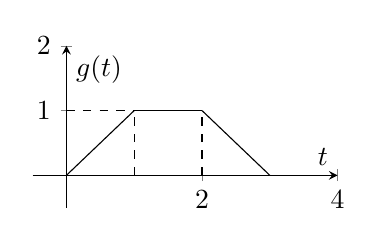
\begin{tikzpicture}[>=stealth]
    \begin{axis}[
        xmin=-.5,xmax=4,
        ymin=-.5,ymax=2,
        axis x line=middle,
        axis y line=middle,
        axis line style=->,
        xlabel={$t$},
        ylabel={$g(t)$},
        width=0.45\textwidth,
        height=0.3\textwidth,
        ]
        \addplot[no marks,black, dashed]coordinates {(0,1)(1,1)};
        \addplot[no marks,black,-]coordinates {(0,0)(1,1)};
        \addplot[no marks,black, dashed]coordinates {(1,0)(1,1)};
        \addplot[no marks,black,-]coordinates {(1,1)(2,1)};
        \addplot[no marks,black, dashed]coordinates {(2,0)(2,1)};
        \addplot[no marks,black,-]coordinates {(2,1)(3,0)};
    \end{axis}
\end{tikzpicture}
\end{figure}

\section*{Problem 2}
Let $v_1=\begin{bmatrix} 1 \\ 3 \\ 5 \end{bmatrix}$,$v_1=\begin{bmatrix} 2 \\ 5 \\ 9 \end{bmatrix}$,$v_1=\begin{bmatrix} -3 \\ 9 \\ 3 \end{bmatrix}$,
\begin{enumerate}[1)]
\item Determine if $\{v_1,v_2,v_3\}$ is linearly independent?
\newline
\item If it is linearly independent find $a$, $b$, $c$ where $av_1 + bv_2 + cv_3 = 0$.
If not, find the relations among $v_1,v_2,v_3$.
\newline
\end{enumerate}

\section*{Problem 3}
Given 5 equations:
\begin{align*}
 2a + b &= 20 \\
 6a + b &= 18 \\
20a + b &= 10 \\
30a + b &=  6 \\
40a + b &=  2 \\
\end{align*}
\begin{enumerate}[a)]
\item Find the closest solution $\{a,b\}$ to the five equations.
{\color{blue} Use MATLAB to confirm how "close" it is.}
\newline
\item Is there any geometric meaning for $\{a,b\}$?
\newline
\end{enumerate}

\section*{Problem 4}
Using the transfer function $\frac{Y(s)}{R(s)} = \frac{6}{(s+2)(s+3)}$.
\newline
Note this transfer function has no zero/pole cancellation and is a minimal polynomial.
\begin{enumerate}[1)]
\item Convert from Transfer function to Differential equation then to the State equations.
\newline
\item Confirm by converting diretly from the Transfer function to the State equation.
{\color{blue} Use MATLAB to confirm.}
\newline
\item Calculate the impulse respone of the system.
\newline
\end{enumerate}

\section*{Problem 5}
Use the Cayley Hamilton Theorem to find $A^{-1}$ where $A = \begin{bmatrix} 0 & 1 \\ -2 & 3 \end{bmatrix}$.
Validate your answer with $AA^{-1}$.
\newline

\section*{Problem 6}
Given the following system with initial conditions:
\begin{align*}
\frac{dx}{dt} &= \begin{bmatrix} -2 & 0 \\ 0 & -4 \end{bmatrix} x(t) + \begin{bmatrix} 4 \\ -1 \end{bmatrix} r(t) \\
y(t) &= \begin{bmatrix} 1 & 3 \end{bmatrix} x(t) \\
x(0) &= \begin{bmatrix} 4 \\ 5 \end{bmatrix} \\
\end{align*}
\begin{enumerate}[a)]
\item Find the state trasition matrix $\varphi (t) = e^{At}$. 
{\color{blue} Use MATLAB to confirm}
\newline

\item Find the transfer function $\frac{Y(s)}{R(s)}$ (factor all polynomials).
\newline
\item Find the total solution for the state vector $x(t)$ if the input $r(t) = 2 u(t)$ where $u(t) = unit step function$.
{\color{blue} Use MATLAB to confirm}
\newline
\hspace*{10mm} Clearly identify the \textbf{zero input part} of the solution
\newline
\hspace*{10mm} Clearly identify the \textbf{zero state part} of the solution
\newline
\hspace*{10mm} Then combine into a final result
\newline
Show the results in both the time domain and Laplace domain.
\textbf{Hint:} It is easier to solve if you work in the Laplace domain then convert to the time domain.
\end{enumerate}
\end{document}
